%% eval.tex
%% $Id: eval.tex 5 2005-10-10 20:55:48Z bless $

\chapter{Evaluation}
\label{ch:Evaluation}
Die Evaluation der Ergebnisse beginnt damit, die Daten der eSense Earpods in Fenster (\textit{windows}) einzuteilen.
Auf diese Fenster werden anschließend \textit{Features} berechnet, welche die Grundlage für die Klassifizierung sind.

\section{Gibt es passende Features?}
Die Suche nach passenden Features wird mit dem Python Package \texttt{tsfresh} angegangen.
\texttt{tsfresh} berechnet automatisch Charakteristiken, sowie deren Relevanz anhand eines Zeitintervalls (\textit{Feature}) \cite{TsfreshTsfresh12}.
Diese Charakteristiken werden fortan als Features bezeichnet.

Wie in Kapitel \ref{ch:Implementierung:classification_pipeline} bereits erklärt, wird eine Messung in viele sich überlappende Fenster aufgeteilt. 
Eine Messung wird in eine Fenstergröße von $5\si{\s}$, bzw. $10\si{\s}$ und einer Verschiebung des nächsten Fensters von $1\si{\s}$ in viele Teile aufgeteilt. 
Nun wird für jedes Fenster eine Featureberechnung ausgeführt, womit durch \texttt{tsfresh} ($\sim$ 6000) Features für jedes Fenster entstehen.
Als Eingabe bekommt \texttt{tsfresh} die Daten der eSense Earpods, also die \textit{x, y} und \textit{z}- Achse der Gyroskop und Beschleunigungsdaten, versehen mit einem Zeitstempel. 

\section{Ablauf der Evaluierung}
Im Kapitel \ref{ch:Implementierung:classification_pipeline} wurde beschrieben, wie die Features berechnet und persistiert wurden. 
Nun sind pro Studienteilnehmer für alle 3 Positionen Features berechnet worden. 
Es sind jeweils die Features für ein Fenster von 5 Sekunden und 10 Sekunden berechnet worden.
Zur Erinnerung: Jede Messung wurde in Fenster der Länge von 5, bzw. 10 Sekunden aufgeteilt, wobei jedes Fenster um eine Sekunde verschoben ist.

\subsection{Data Labeling}
Zur Klassifikation müssen die Daten bereits markiert sein, um eine Entscheidung treffen zu können. 
Beim Abspeichern der eSense Daten ist dies bereits geschehen. 
Da die Messung genau vorgibt, wann eine Person die luft anhalten soll, beziehungsweise nicht, wird diese Information mit einem \textit{Boolean} als zusätzliches Attribut vermerkt.
Da bei der Klassifikation Features anhand der eSense Daten berechnet werden, darf dieses Attribut offensichtlich nicht Teil der Featureberechnung sein.
Da nun bei einem 5 Sekunden Intervall circa 250 Einträge, bei einem 10 Sekunden Intervall circa 500 Einträge in eine Featureberechnung zusammenfließen, muss die Markierung dieses Features gewählt werden.
Ab 50\% der markierten Einträge wird das ganze Intervall als markiert gesetzt.
Dies ist eine essenzielle Entscheidung, da beim Training des Modells nun anhand dieser Markierung entschieden wird, ob ein Intervall ein Atemaussetzer repräsentiert, oder nicht.
\todo{genauer beschreiben, warum hier 50\% gewählt wurde... ich wollte bei 90\% z.B die Übergänge nicht als 0 markieren, weil dann teile der 0 markierten features eigentlich ein Atemaussetzer gewesen wäre... dann trainiert es kacke...}
Nun können die Resultate mit den Klassifikatoren verglichen werden.

\subsection{Kreuzvalidierungsverfahren}
\subsubsection{Within Subject (\textit{k-fold cross validation})}
Das erste Kreuzvalidierungsverfahren ist die \textit{K-fold cross validation}.
Bei diesem Verfahren werden alle Daten in $k$ Partitionen aufgeteilt.
Eine Partition wird als Testdatensatz und $k-1$ Partitionen werden als Trainingsdatensatz gewählt \cite{neumannMaschineLearningKIT2020}.
Somit werden alle Personen als ein Datensatz zusammengefasst und mit der Methode \texttt{test\_train\_split} in Trainingsdaten und Testdaten aufgeteilt.
Hier wird eine Aufteilung von 70\% für die Trainingsdaten und 30\% für die Testdaten gewählt. 
Daraus ergibt sich ein \textit{score}, welcher \todo{was gibt mit der score}
Die Resultate sind in Abbildung \ref{evaluation:within_subject_results} zu sehen.

\begin{table}[H]
  \begin{tabular}{cc}
    \begin{minipage}{1\textwidth}
      \begin{center}
          \begin{tabular}{ | l | c | c | c | c | c | }
            \hline
            \textbf{Verfahren} & \textbf{Positionen} & \textbf{Score} & \textbf{Score} & \textbf{Score} & \textbf{Score} \\ 
            & & \textbf{$w=5\si{\s}$} & \textbf{$w=5\si{\s}$} & \textbf{$w=10\si{\s}$} & \textbf{$w=10\si{\s}$} \\
            & & \textbf{$d=1\si{\s}$} & \textbf{$d=5\si{\s}$} & \textbf{$d=1\si{\s}$} & \textbf{$d=10\si{\s}$} \\ \hline
            Random Forest & Alle &  0.87 & 0.74 & 0.89 & 0.71 \\ 
             & Rücken & 0.85 & 0.67 & 0.93 & 0.57 \\
             & Seite  & 0.86 & 0.72 & 0.89 & 0.75 \\
             & Bauch  & 0.90 & 0.85 & 0.92 & 0.66 \\ \hline
            XG Boost  & Alle & 0.88 & 0.70 & 0.92 & 0.76 \\ 
             & Rücken & 0.89 & 0.67 & 0.95 & 0.62 \\
             & Seite  & 0.90 & 0.78 & 0.92 & 0.48 \\
             & Bauch  & 0.90 & 0.75 & 0.95 & 0.63 \\ \hline
            SVM & Alle& 0.54 & 0.48 & 0.65 & 0.42 \\ 
             & Rücken & 0.60 & 0.67 & 0.72 & 0.46 \\
             & Seite  & 0.57 & 0.38 & 0.63 & 0.5 \\
             & Bauch  & 0.61 & 0.41 & 0.67 & 0.4 \\
            \hline
          \end{tabular}
      \end{center}
    \end{minipage}
  \end{tabular}

  \caption{Ergebnisse des Kreuzvalidierungsverfahrens innerhalb eines Subjects mit einer Aufteilung von 70\% Trainings- und 30\% Testdaten. Alle Personen der Nutzerstudie wurden verwendet. $w$ steht für die Fenstergröße, $d$ für die Verschiebung der aneinanderfolgenden Fenster.}
  \label{evaluation:within_subject_results}
\end{table}

Die Tabelle zeigt die Ergebnisse verschiedener Klassifikationsalgorithmen mit verschiedenen Datensätzen.
Pro Klassifikationsalgorithmus wurden alle Positionen, sowie jede Position einzeln betrachtet, d.h jede Position jeder Person.
Jede Kombination aus Klassifikationsalgorithmus und gewähltem Datensatz wurde nun mit den Fenstergrößen von $5\si{\s}$ und $10\si{\s}$ mit einer Verschiebung von $1\si{\s}$ und einer Verschiebung der Fenstergröße evaluiert.
Somit wurden die Fenstergrößen mit und ohne überlappende Fenster getestet.
Die Resultate zeigen, dass der \textit{score} mit überlappenden Fenstern deutlich höher ist.
Dies könnte daran liegen, dass deutlich mehr Fenster pro Datensatz existieren, falls eine Überlappung der aneinanderfolgenden Fenster stattfindet.
Jedoch ist es auch möglich, dass Teile der überlappenden Fenster bereits erkannt und markiert wurden.
Dadurch ist der überlappende Teil eventuell in den Trainingsdaten vorhanden und eine Klassifizierung ist einfach für den Klassifikationsalgorithmus.

\subsubsection{Leave One Subject Out (LOSO)}
Neben dem k-fachen Kreuzvalidierungsverfahren wird das das \textit{Leave One Subject Out} (\textit{LOSO}) Kreuzvalidierungsverfahren herbeigezogen. 
Hierbei wird ein Modell anhand der Daten der Studienteilnehmer trainiert, jedoch wird ein Datensatz eines Studienteilnehmers ausgelassen. 
Dieser eine Datensatz wird schließlich verwendet, um eine Vorhersage anhand der Trainingsdaten zu treffen, ohne durch interne Trainingsdaten optimiert sein zu können.
Im Folgenden wurde das LOSO Kreuzvalidierungsverfahren mit den beiden Klassifikationsalgorithmen \textit{Random Forest} und \textit{XGBoost} durchgeführt. 
Es wurde jede Person einmal ausgelassen und auf den Trainingsdatensatz angewandt, welcher diese Person nicht enthält. 
Somit entstehen 7 Resultate, von denen nun der Mittelwert gebildet wird.
Die Resultate sind in den Abbildungen \ref{evaluation:random_forest_loso:person6} und \ref{evaluation:xgboost_loso:person6} beispielhaft an Person 6 dargestellt.
Im Anhang sind weitere Abbildungen anderer Personen zu finden.
Die Abbildungen listen die Häufigkeit der Vorhersagen für jede einzelne Sekunde. 
Da eine Sekunde aufgrund der überlappender Fenster in mehreren Fenstern vorkommt, summieren sich die Vorhersagen pro Sekunde maximal auf die Fenstergröße.
Zu Erkennen ist, dass die Fenstergröße von $10\si{\s}$ deutlich bessere Ergebnisse liefert, als eine Fenstergröße von $5\si{\s}$. 
XGBoost neigt bei einer Fenstergröße von $5\si{\s}$ zum Overfitting, ebenso wie Random Forest. 
Da bei der Nutzerstudie die 3 Phasen des Luftanhaltens $10\si{\s}$, $20\si{\s}$, bzw $30\si{\s}$ betrag, könnte dies \todo{ein möglicher Grund sein, kp warum aber :D}
Der Mittelwert aller Ergebnisse des LOSO Kreuzvalidierungsverfahrens sind im \textit{Precision} und \textit{Recall} der unterliegenden Tabelle der Beispiele bei Person 6 mit dem Mittelwert zusammengetragen worden. 
Zu sehen ist, dass XGBoost bessere Ergebnisse liefert als Random Forest.
\todo{schreibe darüber, was die ergebnisse von LOSO aussagen} \newline
Des weiteren, um mögliche Positionsabhängigkeiten zu erkennen, wurden das selbe erneut evaluiert, jedoch nur mit den einzelnen Positionsdaten der jeweiligen Person. 
In der Tabelle \ref{evaluation:loso_classification_results} sind die Resultate zu sehen.
\todo{schreibe darüber, was die ergebnisse der einzelnen personen aussagen}

\subsection{Relevante Features}
Jede Klassifikation ergab ein Resultat, welches durch einzelne Features entschieden wurde. 
Das Python-Framework \texttt{scikit-learn} beinhaltet \texttt{feature\_importances\_} zeigt die Relevanz der einzelnen Features in einem Plot.
Um einen kleinen Überblick zu bekommen, welche Features entscheidend für die Evaluation waren, sind nun einige aufgelistet.
\begin{itemize}
    \item \texttt{gyroZ partial autocorrelation}
    \item \texttt{gytoX fft coefficient}
    \item \texttt{gyroX agg autocorrelation}
    \item \texttt{accY autocorrelation}
    \item \texttt{gyroY change quantiles }
    \item \texttt{gyroZ fft coefficient}
\end{itemize}
Diese Features wurden mittels \texttt{tsfresh} berechnet und waren bei der Klassifikation des Kreuzvalidierungsverfahrens entscheidened \cite{TsfreshTsfresh12}.
Die partielle Autokorrelationfunktion (\texttt{partial autocorrelation}) beschreibt die Abhänigkeit zwischen den Werten der Zeitreihen. 
Zudem wird ein zeitlicher linearer Zusammenhang der verschiedenen Werte gemessen.
Somit haben sich die Werte in diesem Fenster zwischen den Werten vermutlich weniger verändert und ähneln somit eher den positiv markierten Trainingsdaten.

Die \textit{Schnelle Fourier-Transformation} berechnet effizient die diskrete Fourier-Transformation.
Damit können zeidiskrete Signale in Frequenzanteile zerlegt werden. 
Es wird aus einer Darstellung, bestehend aus Zeit- und Abtastwert in eine Darstellung, bestehend aus Frequenzanteil, Amplitude und Phase überführt.
Die Funktion \texttt{fft\_coefficient} in \texttt{tsfresh} berechnet die Fourier Koeffizienten einer eindimensionalen diskreten Fouriertransformation für eine reale Eingabe mit dem Algorithmus der Fast-Fourier-Transformation:
\[A_k = \sum_{m=0}^{n-1} a_m \exp ^ {-2\pi i \frac{mk}{n}}, \hspace{1cm} k = 0,\dots,n-1\]
Die bei der Apnoephase geringe Amplitude ist hier erkennbar und detektierbar, womit eine Klassifikation ermöglicht wird.
Die Aggregation \texttt{agg\_autocorrelation} berechnet den Wert der Autokorrelationsfunktion $f_{agg}$ (beispielsweise die Varianz oder den Mittelwert) über die Autokorrelation $R(l)$ für die verschiedenen Fenster. 
\[R(l) = \frac{1}{(n-l)\sigma ^2} \sum_{t=1}^{n-l} (X_t - \mu) (X_{t+l} - \mu)\]
$X_i$ sind hierbei  die Werte der Timeseries, $n$ deren Länge. 
$\sigma$ und $\mu$ sind Schätzwerte für die Varianz und den Mittelwert.

Ein weiteres Feature, welches ausschlaggebend für die Klassifikation ist, ist der Wechsel der Quantilwerte (\texttt{change\_quantiles}).
Pro Fenster wird ein $ql$ niedriges Quantil und ein $qh$ hohes Quantil berechnet, anschließend wird der durchschnittliche, absolute Wert der aufeinanderfolgenden Änderungen der Reihe x innerhalb dieser Quantile berechnet.
Dadurch werden starke Veränderungen deutlich und stellen klar, dass in diesem Fenster kein Apnoe stattfindet. 


%%%%%%%%%%%%%%%%%%%        RANDOM FOREST 5 sec %%%%%%%%%%%%%%%%%%%%%%%%%%%%%%%%%
\begin{figure}[H]
  \textbf{Random Forest ($w=5\si{\s}$, $d=1\si{\s}$)}
    \centering
    \begin{subfigure}{1\textwidth}
        \includegraphics[width=1\textwidth]{evaluation/loso_5sec/random_forest_loso/Random Forest (Leave one Subject out: Person 6 back).png}
        %\caption{Resultate der Person 6 auf dem Rücken liegend.}
      \end{subfigure}
      \begin{subfigure}{1\textwidth}
        \includegraphics[width=1\textwidth]{evaluation/loso_5sec/random_forest_loso/Random Forest (Leave one Subject out: Person 6 side).png}
        %\caption{Resultate der Person 6 auf der Seite liegend.}
      \end{subfigure}
      \begin{subfigure}{1\textwidth}
        \includegraphics[width=1\textwidth]{evaluation/loso_5sec/random_forest_loso/Random Forest (Leave one Subject out: Person 6 stomach).png}
        %\caption{Resultate der Person 6 auf dem Bauch liegend.}
    \end{subfigure}
    \begin{subfigure}{1\textwidth}
        \begin{center}
            \begin{tabular}{ | l | c | c | r | }
              \hline
               & precision & recall & f1-score\\ \hline
              0 & 0.92 & 0.75 & \\ \hline
              1 & 0.75 & 0.67 & \\
              \hline
            \end{tabular}
        \end{center}
        \caption{Random Forest mit dem Kreuzvalidierungsverfahren. Die Tabelle zeigt den Mittelwert aller Vorhersagen der einzelnen Personen.}
        \label{implementation:app:screenshots:user_studies_information}
    \end{subfigure}
    \newline
    \vspace*{1 cm}
    \newline
    \textbf{Random Forest ($w=10\si{\s}$, $d=1\si{\s}$)}
    \begin{subfigure}{1\textwidth}
      \includegraphics[width=1\textwidth]{evaluation/loso_10sec/random_forest_loso/Random Forest (Leave one Subject out: Person 6 back).png}
      %\caption{Resultate der Person 6 auf dem Rücken liegend.}
    \end{subfigure}
    \begin{subfigure}{1\textwidth}
      \includegraphics[width=1\textwidth]{evaluation/loso_10sec/random_forest_loso/Random Forest (Leave one Subject out: Person 6 side).png}
      %\caption{Resultate der Person 6 auf der Seite liegend.}
    \end{subfigure}
    \begin{subfigure}{1\textwidth}
      \includegraphics[width=1\textwidth]{evaluation/loso_10sec/random_forest_loso/Random Forest (Leave one Subject out: Person 6 stomach).png}
      %\caption{Resultate der Person 6 auf dem Bauch liegend.}
  \end{subfigure}

  \begin{subfigure}{1\textwidth}
      \begin{center}
          \begin{tabular}{ | l | c | c | r | }
            \hline
             & precision & recall & \\ \hline
            0 & 0.91 & 0.76 & \\ \hline
            1 & 0.76 & 0.67 & \\
            \hline
          \end{tabular}
      \end{center}
      \caption{Random Forest mit dem Kreuzvalidierungsverfahren (LOSO). Die Tabelle zeigt den Mittelwert aller Vorhersagen der einzelnen Personen.}
      \label{implementation:app:screenshots:user_studies_information}
  \end{subfigure}
    \caption{Das Kreuzvalidierungsverfahren (LOSO) mit dem Klassifikationsalgorithmus Random Forest. Das Modell wurde auf allen Personen, exklusive einer Person trainiert und auf alle Positionen dieser einen Person wurde eine Vorhersage getroffen. Am Beispiel hier sind die Resultate von Person 6 zu sehen. Die blauen Bereiche sind die, in denen die Luft angehalten wurde, die orangene Kurve ist die Vorhersage. ($w=$ Fenstergröße, $d=$ Verschiebung der Fenster)}
\label{evaluation:random_forest_loso:person6}
\end{figure}

%%%%%%%%%%%%%%%%%%%        XG BOOST 5 sec %%%%%%%%%%%%%%%%%%%%%%%%%%%%%%%%%

\begin{figure}[H]
  \textbf{XG Boost ($w=5\si{\s}$, $d=1\si{\s}$)}
    \centering
    \begin{subfigure}{1\textwidth}
        \includegraphics[width=1\textwidth]{evaluation/loso_5sec/xg_boost_loso/XG Boost (Leave one Subject out: Person 6 back).png}
        %\caption{Resultate der Person 6 auf dem Rücken liegend.}
      \end{subfigure}
      \begin{subfigure}{1\textwidth}
        \includegraphics[width=1\textwidth]{evaluation/loso_5sec/xg_boost_loso/XG Boost (Leave one Subject out: Person 6 side).png}
        %\caption{Resultate der Person 6 auf der Seite liegend.}
      \end{subfigure}
      \begin{subfigure}{1\textwidth}
        \includegraphics[width=1\textwidth]{evaluation/loso_5sec/xg_boost_loso/XG Boost (Leave one Subject out: Person 6 stomach).png}
        %\caption{Resultate der Person 6 auf dem Bauch liegend.}
    \end{subfigure}

    \begin{subfigure}{1\textwidth}
        \begin{center}
            \begin{tabular}{ | l | c | c | r | }
              \hline
               & precision & recall & f1-score \\ \hline
              0 & 0.93 & 0.70 & 0.0 \\ \hline
              1 & 0.70 & 0.73 & 0.0 \\
              \hline
            \end{tabular}
        \end{center}
        \caption{XGBoost mit dem Kreuzvalidierungsverfahren (LOSO). Die Tabelle zeigt den Mittelwert aller Vorhersagen der einzelnen Personen.}
        \label{implementation:app:screenshots:user_studies_information}
    \end{subfigure}
    \newline
    \vspace*{1 cm}
    \newline
    \textbf{XG Boost ($w=10\si{\s}$, $d=1\si{\s}$)}
    \begin{subfigure}{1\textwidth}
      \includegraphics[width=1\textwidth]{evaluation/loso_10sec/xg_boost_loso/XG Boost (Leave one Subject out: Person 6 back).png}
      %\caption{Klassifikationsresultate der Person 6. Die Messung wurde auf dem Rücken liegend durchgeführt.}
    \end{subfigure}
    \begin{subfigure}{1\textwidth}
      \includegraphics[width=1\textwidth]{evaluation/loso_10sec/xg_boost_loso/XG Boost (Leave one Subject out: Person 6 side).png}
      %\caption{Klassifikationsresultate der Person 6. Die Messung wurde auf der Seite liegend durchgeführt.}
    \end{subfigure}
    \begin{subfigure}{1\textwidth}
      \includegraphics[width=1\textwidth]{evaluation/loso_10sec/xg_boost_loso/XG Boost (Leave one Subject out: Person 6 stomach).png}
      %\caption{Klassifikationsresultate der Person 6. Die Messung wurde auf dem Bauch liegend durchgeführt.}
  \end{subfigure}

  \begin{subfigure}{1\textwidth}
      \begin{center}
          \begin{tabular}{ | l | c | c | r | }
            \hline
             & precision & recall & f1-score \\ \hline
            0 & 0.93 & 0.74 & 0.0 \\ \hline
            1 & 0.74 & 0.75 & 0.0 \\
            \hline
          \end{tabular}
      \end{center}
      \caption{XGBoost mit dem Kreuzvalidierungsverfahren (LOSO). Die Tabelle zeigt den Mittelwert aller Vorhersagen der einzelnen Personen.}
      \label{implementation:app:screenshots:user_studies_information}
  \end{subfigure}
    \caption{Das Kreuzvalidierungsverfahren (LOSO) mit dem Klassifikationsalgorithmus XG Boost. Das Modell wurde auf allen Personen, exklusive einer Person trainiert und auf alle Positionen dieser einen Person wurde eine Vorhersage getroffen. Am Beispiel hier sind die Resultate von Person 6 zu sehen. Die blauen Bereiche sind die, in denen die Luft angehalten wurde, die orangene Kurve ist die Vorhersage. ($w=$ Fenstergröße, $d=$ Verschiebung der Fenster)}
\label{evaluation:xgboost_loso:person6}
\end{figure}

%%%%%%%%%%%%%%%%%%%        Position based results  5 sec %%%%%%%%%%%%%%%%%%%%%%%%%%%%%%%%%
\begin{table}
\begin{tabular}{cc}    
    \begin{minipage}{.33\linewidth}
        \begin{center}
            \begin{tabular}{ | l | c | c | r | }
              \hline
               & precision & recall & f1-score \\ \hline
              0 & 0.90 & 0.72 & 0.0 \\ \hline
              1 & 0.72 & 0.57 & 0.0 \\
              \hline
            \end{tabular}
            \smallskip
            \\ Random Forest (only side, \textit{window: 5s})
        \end{center}
        %\label{evaluation:5s:random_forest_loso_side}
    \end{minipage}

    \begin{minipage}{.33\linewidth}
        \begin{center}
            \begin{tabular}{ | l | c | c | r | }
              \hline
               & precision & recall & f1-score \\ \hline
              0 & 0.89 & 0.83 & 0.0 \\ \hline
              1 & 0.83 & 0.45 & 0.0 \\
              \hline
            \end{tabular}
            \smallskip
            \\ Random Forest (only back, \textit{window: 5s})
        \end{center}
        %\label{evaluation:5s:random_forest_loso_back}
    \end{minipage}

    \begin{minipage}{0.33\textwidth}
        \begin{center}
            \begin{tabular}{ | l | c | c | r | }
              \hline
               & precision & recall & f1-score \\ \hline
              0 & 0.92 & 0.72 & 0.0 \\ \hline
              1 & 0.72 & 0.66 & 0.0 \\
              \hline
            \end{tabular}
            \smallskip
            \\ Random Forest (only stomach, \textit{window: 5s})
        \end{center}
        %\label{evaluation:5s:random_forest_loso_stomach}
    \end{minipage}
\end{tabular}
\newline
\vspace*{5mm}
\newline
\begin{tabular}{cc}
    \begin{minipage}{0.33\textwidth}
        \begin{center}
            \begin{tabular}{ | l | c | c | r | }
              \hline
               & precision & recall & f1-score \\ \hline
              0 & 0.91 & 0.67 & 0.0 \\ \hline
              1 & 0.67 & 0.61 & 0.0 \\
              \hline
            \end{tabular}
            \smallskip
            \\ XG Boost (only side, \textit{window: 5s})
        \end{center}
        %\label{evaluation:5s:xg_boost_loso_side}
    \end{minipage}

    \begin{minipage}{0.33\textwidth}
        \begin{center}
            \begin{tabular}{ | l | c | c | r | }
              \hline
               & precision & recall & f1-score \\ \hline
              0 & 0.90 & 0.75 & 0.0 \\ \hline
              1 & 0.75 & 0.54 & 0.0 \\
              \hline
            \end{tabular}
            \smallskip
            \\ XG Boost (only back, \textit{window: 5s})
        \end{center}
        %\label{evaluation:5s:xg_boost_loso_back}
    \end{minipage}

    \begin{minipage}{0.33\textwidth}
        \begin{center}
            \begin{tabular}{ | l | c | c | r | }
              \hline
               & precision & recall & f1-score \\ \hline
              0 & 0.94 & 0.71 & 0.0 \\ \hline
              1 & 0.71 & 0.72 & 0.0 \\
              \hline
            \end{tabular}
            \smallskip 
            \\ XG Boost (only stomach, \textit{window: 5s})
        \end{center}
        %\label{evaluation:5s:xg_boost_loso_stomach}
    \end{minipage}
\end{tabular}
\newline
\vspace*{5mm}
\newline
%%%%%%%%%%%%%%%%%%%        Position based results  10 sec %%%%%%%%%%%%%%%%%%%%%%%%%%%%%%%%%
  \begin{tabular}{cc}    
      \begin{minipage}{.33\linewidth}
          \begin{center}
              \begin{tabular}{ | l | c | c | r | }
                \hline
                 & precision & recall & f1-score \\ \hline
                0 & 0.89 & 0.79 & 0.0 \\ \hline
                1 & 0.79 & 0.53 & 0.0 \\
                \hline
              \end{tabular}
              \smallskip
              \\ Random Forest (only side, \textit{window: 10s})
          \end{center}
          %\label{evaluation:5s:random_forest_loso_side}
      \end{minipage}
  
      \begin{minipage}{.33\linewidth}
          \begin{center}
              \begin{tabular}{ | l | c | c | r | }
                \hline
                 & precision & recall & f1-score \\ \hline
                0 & 0.89 & 0.79 & 0.0 \\ \hline
                1 & 0.79 & 0.52 & 0.0 \\
                \hline
              \end{tabular}
              \smallskip
              \\ Random Forest (only back, \textit{window: 10s})
          \end{center}
          %\label{evaluation:5s:random_forest_loso_back}
      \end{minipage}
 
      \begin{minipage}{0.33\textwidth}
          \begin{center}
              \begin{tabular}{ | l | c | c | r | }
                \hline
                 & precision & recall & f1-score \\ \hline
                0 & 0.94 & 0.71 & 0.0 \\ \hline
                1 & 0.71 & 0.73 & 0.0 \\
                \hline
              \end{tabular}
              \smallskip
              \\ Random Forest (only stomach, \textit{window: 10s})
          \end{center}
          %\label{evaluation:5s:random_forest_loso_stomach}
      \end{minipage}
  \end{tabular}
  \newline
  \vspace*{5mm}
  \newline
  \begin{tabular}{cc}
      \begin{minipage}{0.33\textwidth}
          \begin{center}
              \begin{tabular}{ | l | c | c | r | }
                \hline
                 & precision & recall f1-score \\ \hline
                0 & 0.90 & 0.78 & 0.0 \\ \hline
                1 & 0.78 & 0.61 & 0.0 \\
                \hline
              \end{tabular}
              \smallskip
              \\ XG Boost (only side, \textit{window: 10s})
          \end{center}
          %\label{evaluation:5s:xg_boost_loso_side}
      \end{minipage}

      \begin{minipage}{0.33\textwidth}
          \begin{center}
              \begin{tabular}{ | l | c | c | r | }
                \hline
                 & precision & recall f1-score \\ \hline
                0 & 0.90 & 0.75 & 0.0 \\ \hline
                1 & 0.75 & 0.58 & 0.0 \\
                \hline
              \end{tabular}
              \smallskip
              \\ XG Boost (only back, \textit{window: 10s})
          \end{center}
          %\label{evaluation:5s:xg_boost_loso_back}
      \end{minipage}
  
      \begin{minipage}{0.33\textwidth}
          \begin{center}
              \begin{tabular}{ | l | c | c | r |}
                \hline
                 & precision & recall & f1-score \\ \hline
                0 & 0.94 & 0.71 & 0.0 \\ \hline
                1 & 0.71 & 0.72 & 0.0 \\
                \hline
              \end{tabular}
              \smallskip 
              \\ XG Boost (only stomach, \textit{window: 10s})
          \end{center}
          %\label{evaluation:5s:xg_boost_loso_stomach}
      \end{minipage}
  \end{tabular}
  \caption{Klassifikationsergebnisse mit dem Kreuzvalidierungsverfahren bei einer Fenstergröße von 5, bzw. 10 Sekunden, welche um 1 Sekunde verschoben wurden. Es wurde immer eine Person aus dem Trainieren des Modells ausgelassen und auf diese Person wurde anschließend eine Vorhersage getroffen. Jede Person wurde einmel in dem Modell außen vorgelassen und auf dieses Modell vorhergesagt. Das zu sehende Resultat ist der Mittelwert aller Resultate des Kreuzvalidierungsverfahrens der einzelnen Positionen der Position.}
  \label{evaluation:loso_classification_results}
  \end{table}

  % \todo{ich habe gelernt}
% \begin{itemize}
%     \item auswertungsdaten: Auf dem rücken liegende ddaten sind am vielversprechendsten
%     \item die atempausen können einigermaßen klassifiziert werden
%     \item rauschen entfernen bringt nix vermutlich wegen tsfresh, da es das schon macht, also es kommen
%     \item 10 sekunden window size ist besser als 5 sekunden window size
%     \item xgboost bringt bessere resultate, als random forest und svm, braucht aber auch länger
% \end{itemize}

% gibt earables, die blutsauerstoff und puls mittracken können
% plus grafik telegram tobi